\documentclass{beamer}
\usepackage{tcolorbox}
\usepackage{amsmath}
\usepackage{tikz}
\usepackage{pgfplots}
\usepackage{adjustbox}
\usepackage{pdfpages}


%\beamerdefaultoverlayspecification{<+->}
\newcommand{\data}{\mathcal{D}}

\DeclareMathOperator*{\argmin}{arg\,min}

\newcommand\Item[1][]{%
	\ifx\relax#1\relax  \item \else \item[#1] \fi
	\abovedisplayskip=0pt\abovedisplayshortskip=0pt~\vspace*{-\baselineskip}}


\usetheme{metropolis}           % Use metropolis theme


\title{Maths for ML III}
\date{\today}
\author{Nipun Batra}
\institute{IIT Gandhinagar}
\begin{document}
  \maketitle
  
  
  



% \begin{frame}{Contour PLots and Gradients}
    
    
%     Assume f(x,y) = $x^{2}+y^{2}$.\\
    
    
%     \begin{equation*}
%         \nabla f(x,y) = \begin{bmatrix}
%             \frac{\partial }{\partial x} f(x,y)\\
%             \frac{\partial }{\partial y} f(x,y)
%         \end{bmatrix}
%     \end{equation*}
    
%     \begin{equation*}
%         \nabla f(x,y) = 
%         2
%         \begin{bmatrix}
%         x\\
%         y
%         \end{bmatrix}
%     \end{equation*}
    
% \end{frame}


\begin{frame}{Constrained Optimization}

Extreme (max or min) $f(x,y) = x^{2}+y^{2}$ s.t $xy=1$\\

\vspace{2em}
More generally Extrema f(x,\dots) s.t g(x,\dots) = 0
\pause \begin{center}
	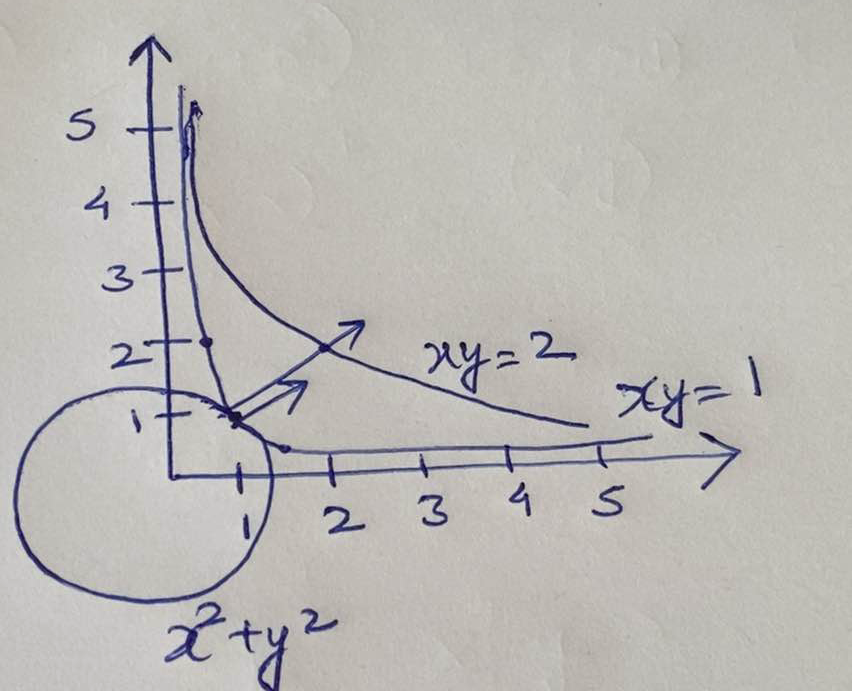
\includegraphics[totalheight=6cm]{ml-maths/constrained.png}
\end{center}



\end{frame}

\begin{frame}{Constrained Optimization}

\begin{tcolorbox}
	At extremum, ($x^*, y^*$), we get: 
$\nabla f(x^*,y^*) = \lambda \nabla g(x^*,y^*)$
\end{tcolorbox}

\pause $\nabla f(x,y) = \begin{bmatrix}
2x\\
2y
\end{bmatrix}
= \lambda \nabla g(x,y)  = \lambda  \begin{bmatrix}
y\\
x\\
\end{bmatrix}$
\end{frame}

\begin{frame}{Constrained Optimization}

\begin{equation}
2x = \lambda y
\end{equation}


\begin{equation}
2y = \lambda x
\end{equation}


\begin{equation}
xy = 1
\end{equation}


\end{frame}

\begin{frame}{Constrained optimization}
We have three equations involving three variables. 
On solving the above equations, we get\\
x = y = 1\\
$\lambda = 2$\\
\end{frame}

\begin{frame}{Constrained Optimization}
Find extrema of $f(x,y) = x^{2} + y^{2}$ s.t $x + y = 1$\\

\end{frame}

\begin{frame}{Constrained Optimization}
$\nabla f(x,y) = \lambda \nabla g(x,y)$ \\
\vspace{1em}
$$
\nabla f(x, y)=\left[\begin{array}{l}
{2 x} \\
{2 y}
\end{array}\right] 
\vspace{1em} 
\nabla g(x, y)=\left[\begin{array}{l}
{1} \\
{1}
\end{array}\right]
$$
\end{frame}

\begin{frame}{Constrained Optimization}
\begin{equation}
2x=\lambda
\end{equation}
\begin{equation}
2y=\lambda
\end{equation}
\begin{equation}
x + y - 1 = 0
\end{equation}
On solving we get x = y = 0.5
\end{frame}


\begin{frame}{Lagrangian Multiplier}
For solving the form of equations: Extrema $f(.)$ s.t. $g(.)$ = 0.

\pause For example, Maximize $f(x, y) = x^2 + y^2$ s.t. $x + y = 1$

\pause Construct a new function, Lagrangian $L(x,y,\lambda) = f(x, y) + \lambda g(x, y)$ where $\lambda$ is called the Lagrangian multiplier 
\pause \begin{itemize}[<+->]
\item Set $\nabla L = 0$, i.e.
\item $\cfrac{\partial L}{\partial x} = 0$
\item $\cfrac{\partial L}{\partial y} = 0$
\item $\cfrac{\partial L}{\partial \lambda} = 0$
\end{itemize}

\end{frame}


\begin{frame}{Lagrangian Multiplier}
Find the extrema of $f(x,y) =x^{2}y$ s.t $g(x,y)=x^{2}+y^{2} = 1$ \\
\vspace{1em}
\pause $L (x, y, \lambda) = x^{2}y + \lambda (x^{2} + y^{2} - 1)$\\
\vspace{1em}
\pause Compute the partial derivatives
\end{frame}

\begin{frame}{Lagrangian Multiplier}
\begin{equation}
\cfrac{\partial L}{\partial x} = 0 \implies 2xy + \lambda(2x) = 0
\end{equation}

\begin{equation}
\cfrac{\partial L}{\partial y} = 0 \implies x^{2} + \lambda(2y) = 0
\end{equation}

\begin{equation}
\cfrac{\partial L}{\partial \lambda} = 0 \implies x^{2} + y^{2} - 1 = 0
\end{equation}
\end{frame}

\begin{frame}{Case 1}
x = 0\\
\vspace{1em}
f(x,y) = 0\\
\vspace{1em}
$y^{2} = 1 \implies y= \pm 1$\\
\vspace{1em}
$\lambda = 0$
\end{frame}

\begin{frame}{Case 2}
x $\neq  0 \implies y = - \lambda$\\
\vspace{1em}
\pause $x^{2} = 2\lambda^{2}$ \\ \pause Substitute the above values in Equation 9\\
\vspace{1em}
\pause $3\lambda^{2} = 1 \implies \lambda = \pm \cfrac{1}{\sqrt{3}}$\\
\vspace{1em}
\pause $y = \pm \cfrac{1}{\sqrt{3}}$\\
\vspace{1em}
Max of $x^{2}y = \cfrac{2}{3} \sqrt{\cfrac{1}{3}}$
\end{frame}


%\begin{frame}{KKT Conditions}
%Minimize f(x)\\
%such that $h_{i} = 0 \hspace{1em} \forall i = 1 \dots m$\\
%such that $g_{i} \leq 0 \hspace{1em} \forall j = 1 \dots n$\\
%
%\begin{equation*}
%L(x,\lambda,\mu)= f(x) + \sum_{i=1}^{n}\lambda_{i}h_{i}(x) + 
%\sum_{i=1}^{m}\mu_{i}g_{i}(x) 
%\end{equation*}
%Now, if $g_{i}(x^{*})<0$, then $\mu_{i}$ can be set to zero.\\
%else  $g_{i}(x^{*})=0$\\
%Therefore $\mu_{i}g_{i}(x^{*})=0 \implies \mu_{i}>0$
%\end{frame}


%\begin{frame}{Lagrange Multiplier}
%Stationarity\\
%\begin{equation*}
%\nabla_{x}f(x) + \sum_{i=1}^{m} \nabla_{x}\lambda_{i}h_{i}(x)+\sum_{i=1}^{m}\nabla_{x}\mu_{i}g_{i}(x)=0
%\end{equation*}
%Equality
%\begin{equation*}
%\nabla_{x}f(\lambda) + \sum_{i=1}^{m} \nabla_{\lambda}\lambda_{i}h_{i}(x)+\sum_{i=1}^{m}\nabla_{\lambda}\mu_{i}g_{i}(x)=0
%\end{equation*}
%Inequality
%\begin{equation*}
%\mu_{i}g_{i}=0 \implies \mu_{i} \geq 0
%\end{equation*}
%\end{frame}


\begin{frame}{KKT Conditions}
	Used for constrained optimization of the form\\
	\vspace{1cm}
	Minimize $f(x)$, where $x \in \mathbb{R}^k$\\
	such that\\
	\begin{center}
		$h_i(x) = 0$,  $\forall i = 1, \dots, m$ (m equalities)\\
		$g_j(x) \leq 0$,  $\forall j = 1, \dots, n$ (n inequalities)\\
	\end{center}
\end{frame}

\begin{frame}{Step 1}
	\begin{itemize}
		\only<1->{
			\item Create a new function for minimization, \\
			\vspace{0.5cm}
			$L(x, \lambda_1, \dots, \lambda_m, \mu_1, \dots, \mu_n ) = f(x) + \sum\limits_{i=1}^{m}\lambda_ih_i(x) + \sum\limits_{j=1}^{n}\mu_jg_j(x)$\\
			\vspace{0.5cm}
			where,\\ $\lambda_1-\lambda_m$ are multipliers for the $m$ equalities \\
			$\mu_1-\mu_n$ are multipliers for the $n$ inequalities \\
		}
	\end{itemize}
\end{frame}

\begin{frame}{Step 2}
	\begin{itemize}
		\item Minimize $L(x, \lambda, \mu)$ w.rt. $x \implies \nabla_xL(x, \lambda, \mu) = 0 $\\
		Gives $k$ equations
	\end{itemize}
\end{frame}

\begin{frame}{Step 3}
	\begin{itemize}
		\item Minimize $L(x, \lambda, \mu)$ w.rt. $\lambda \implies \nabla_\lambda L(x, \lambda, \mu) = 0 $\\
		Gives $m$ equations
	\end{itemize}
\end{frame}

\begin{frame}{Step 4}
	\begin{columns}
		\begin{column}{0.5\textwidth}
			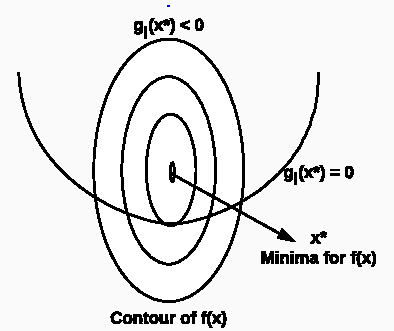
\includegraphics[width = \textwidth]{ml-maths/img1}
			\centering
			$g_i(x^*) \leq 0$\\
			$\mu_i = 0$
		\end{column}
		\begin{column}{0.5\textwidth}
			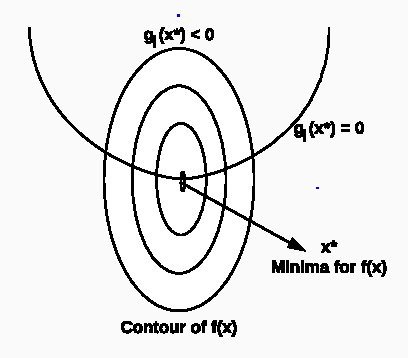
\includegraphics[width = \textwidth]{ml-maths/img2}
			\centering
			$g_i(x^*) = 0$
		\end{column}
	\end{columns}
	\vspace{1cm}
	\centering
	In both cases, $\mu_ig_i(x^*) = 0$
\end{frame}

{
	\setbeamercolor{background canvas}{bg=}
	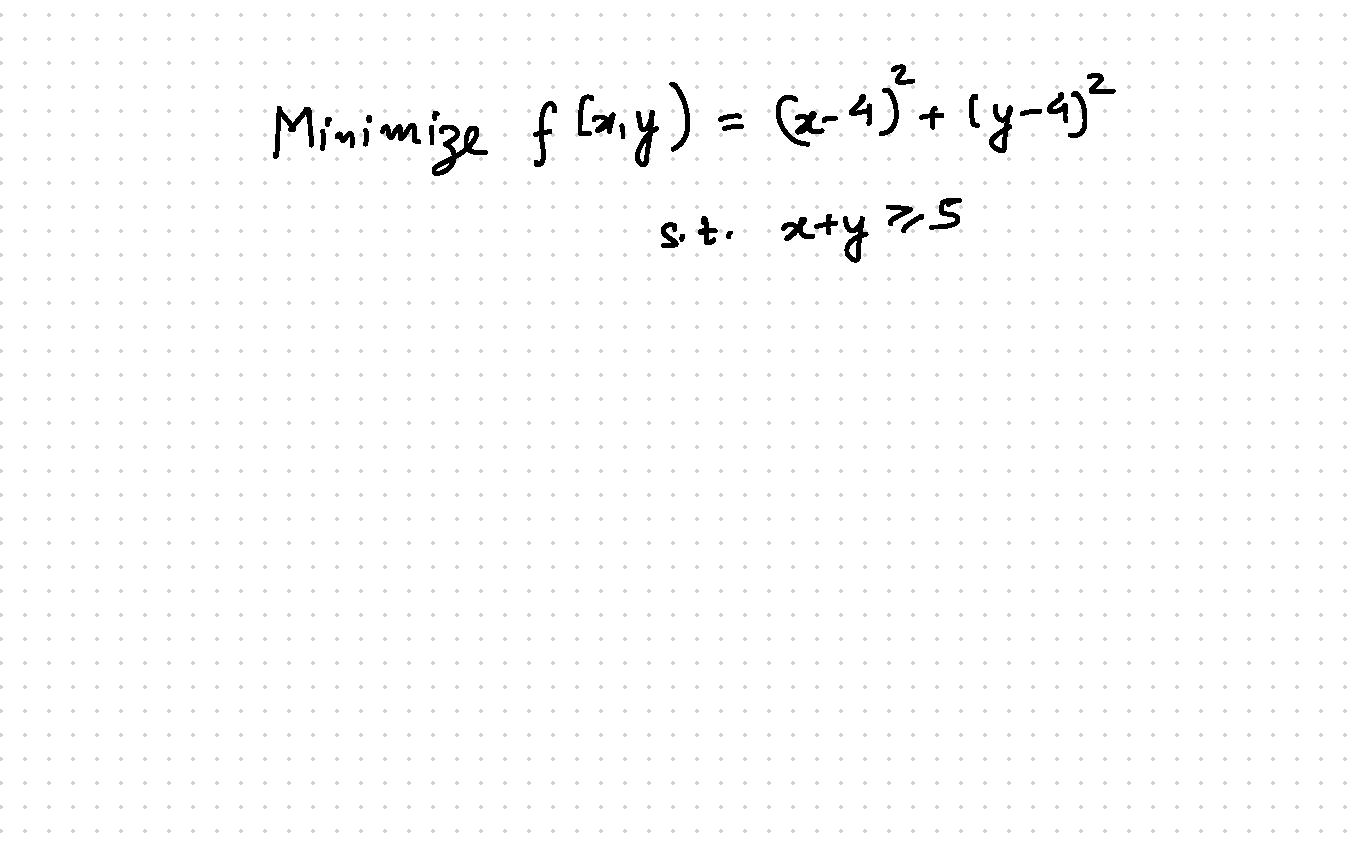
\includepdf[page=-]{kkt-drawing.pdf}
}

%\begin{frame}
%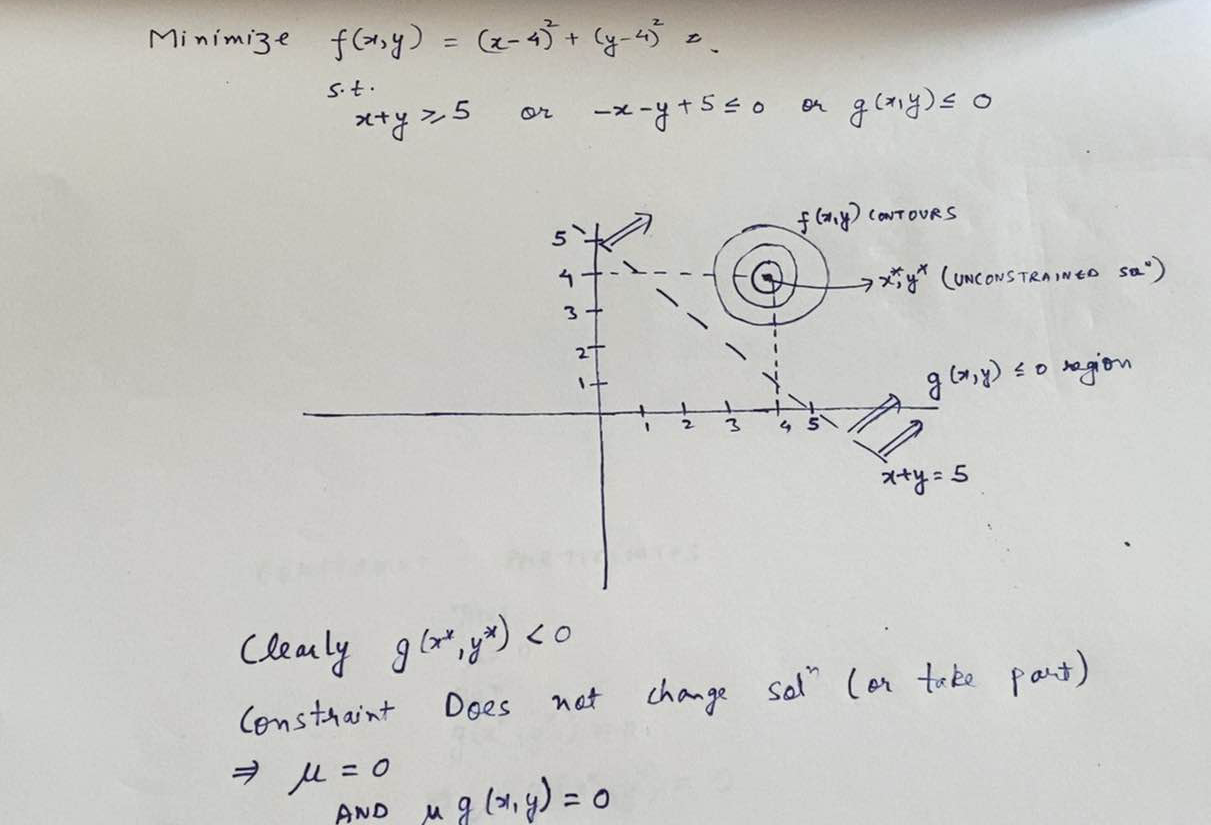
\includegraphics[width=1.1\textwidth]{ml-maths/2.png}
%\end{frame}
%
%\begin{frame}
%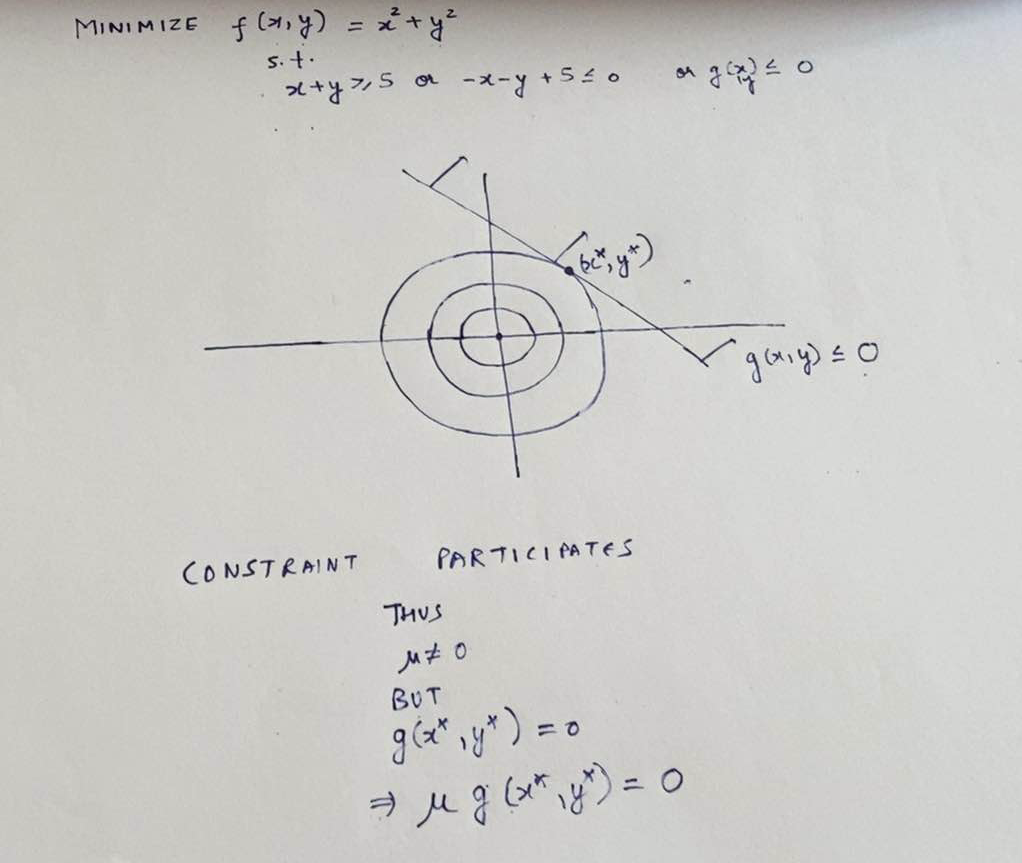
\includegraphics[width=1.1\textwidth]{ml-maths/1.png}
%\end{frame}

%\begin{frame}{Constraint on $\mu_i$'s}
%	\centering
%	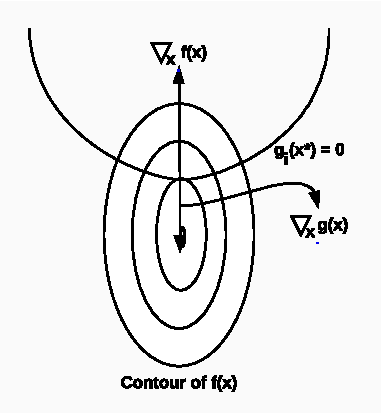
\includegraphics[width = 0.5\textwidth]{ml-maths/img3}
%	$min_xL(x, \lambda, \mu)  \implies \nabla_xf(x) + \nabla_x\mu_ig_i(x) = 0$\\
%	\vspace{0.5cm}
%	$\mu_i = \dfrac{\nabla_xf(x)}{\nabla_x\mu_ig_i(x)} = +ve$
%\end{frame}

\begin{frame}{KKT Conditions}
	\only<1->{
		\textbf{Stationarity (For minimization)}\\
		$\nabla_xf(x) + \sum\limits_{i=1}^m\nabla_x\lambda_ih_i(x)  + \sum\limits_{i=1}^n\nabla_x\mu_ig_i(x) = 0$ \\
		\vspace{0.5cm}
	}
	\only<2->{
		\textbf{Equality Constraints}\\
		$\nabla_\lambda f(x) + \sum\limits_{i=1}^m\nabla_\lambda\lambda_ih_i(x)  + \sum\limits_{i=1}^n\nabla_\lambda\mu_ig_i(x) = 0$ \\
		$\sum\limits_{i=1}^m\nabla_\lambda\lambda_ih_i(x)  = 0$\\
	}
	\only<3->{
		\vspace{0.5cm}
		\textbf{Inequality Constraints (Complementary Slackness)}\\
		$\mu_ig_i(x) = 0 \forall i = 1,\dots, n$\\
		$\mu_i \geq 0$
	}	
\end{frame}

	\begin{frame}{Example}
Minimize $x^2 + y^2$ such that,\\
\centering
$x^2 + y^2 \leq 5$\\
$x + 2y = 4$\\
$x,y \geq 0$
\end{frame}

\begin{frame}{Example}
\only<1->{
$f(x,y) = x^2 + y^2$\\
}
\only<2->{
$h(x,y) = x + 2y - 4$\\
}
\only<3->{
$g_1(x,y) = x^2 + y^2 - 5$\\
}
\only<4->{
$g_2(x,y) = -x$\\
}
\only<5->{
$g_3(x,y) = -y$\\
}
\only<6->{
\vspace{1cm}
$L(x,y, \lambda, \mu_1, \mu_2, \mu_3) = x^2 + y^2 + \lambda(x + 2y - 4) + \mu_1(x^2 + y^2 - 5) + \mu_2(-x) + \mu_3(-y)$\\
}
\end{frame}

\begin{frame}{Example}
\only<1->{
\textbf{Stationarity}\\
$\nabla_xL(x,y, \lambda, \mu_1, \mu_2, \mu_3)  = 0$\\
$\implies 2x + \lambda + 2\mu_1x - \mu_2 = 0 \dots\dots\dots\dots\dots\dots (1)$\\
\vspace{0.5cm}
$\nabla_yL(x,y, \lambda, \mu_1, \mu_2, \mu_3)  = 0$\\
$\implies 2y + 2\lambda + 2\mu_1y - \mu_3 = 0 \dots\dots\dots\dots\dots\dots (2)$\\
}
\only<2->{
\vspace{0.5cm}
\textbf{Equality Constraint}\\
$x + 2y = 4 \dots\dots\dots\dots\dots\dots\dots\dots\dots\dots\dots\dots (3)$\\	
}
\only<3->{
\vspace{0.5cm}
\textbf{Slackness}\\
$\mu_1(x^2 + y^2 - 5) = 0 \dots\dots\dots\dots\dots\dots\dots\dots\dots (4)$\\
$\mu_2x = 0 \dots\dots\dots\dots\dots\dots\dots\dots\dots\dots\dots\dots\dots (5)$\\
$\mu_3y = 0 \dots\dots\dots\dots\dots\dots\dots\dots\dots\dots\dots\dots\dots (6)$
}
\end{frame}

\begin{frame}{Example}
\only<1->{
From (6), $\mu_3 = 0$ or $y = 0$\\
But if, $y = 0$, then $x = 4$ according to (3) . This violates (1).\\
Hence, $y \neq 0$ and $\mu_3 = 0$\\
\vspace{0.5cm}
}
\only<2->{
From (5), $\mu_1 = 0$ or $x = 0$\\
If $x = 0$, $y = 2$, which implies $x^2 + y^2 = 4 (\leq 5)$ \\
Since (x,y) = (0,2) gives smaller $x^2 + y^2$ terms than 5, \\
Using (4), $\mu_1 = 0$\\
}
\only<3->
{
\vspace{0.5cm}
On further solving we get,\\
$x = 0.8$\\
$y = 1.6$\\
}
\end{frame}

{
	\setbeamercolor{background canvas}{bg=}
	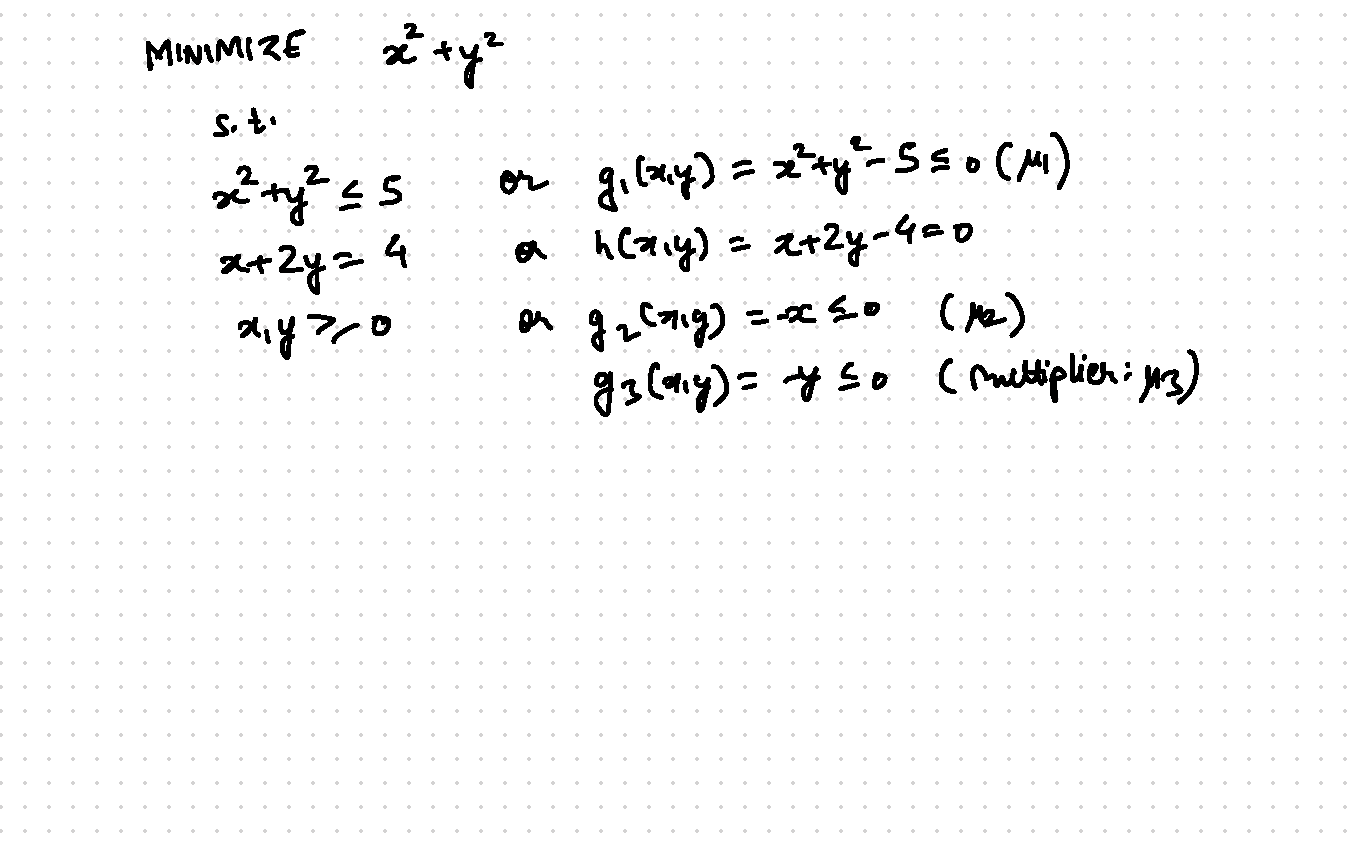
\includepdf[page=-]{constrained-example.pdf}
}

\end{document}